\documentclass{article}

\usepackage{makecell}

% Document extensibility %
%
% Disables native paragraph indentation
\usepackage{parskip} 
%
% Provides further bullet options for lists
\usepackage{enumitem}

% Mathematical symbol and statement packages %
%
% Necessary
\usepackage{amsmath}
\usepackage{amssymb}
%
% Extensive fraction notation
\usepackage{xfrac}
%
% Generic mathematical commands
% Notable: \degree, \celcius
\usepackage{gensymb}
%
% Variable vector notation (arrow above variable)
\usepackage{esvect}
%
% Multiline boxed equations
\usepackage{empheq}
%
% SI Unit
\usepackage{siunitx}

% Graphic packages %
%
% Diagrams and illustrations
\usepackage{tikz}
%
% Image insertion
\usepackage{graphicx}
\graphicspath{ {./} }

% Document content %
%
% Change title of table of contents
% \renewcommand{\contentsname}{Title}

\begin{document}

% Command `\hr` to insert horizontal rules
\newcommand{\hr}{\par\noindent\rule{\textwidth}{0.4pt}}

% Command to box and center math equations
\newcommand{\bc}[1]{
	\begin{equation*}
		\begin{boxed}
			{#1}
		\end{boxed}
	\end{equation*}
}

% Command for single line equations with a condition
\newcommand{\cond}[2]{
	\ifmmode
		{#1} \quad {#2}
	\else
		$$ {#1} \quad {#2} $$
	\fi
}

\tableofcontents

\section{Exercise 5: Photosynthesis \& The Carbon Cycle}

\subsection{Procedure 1}
\textbf{QUESTIONS}
\begin{enumerate}[label=\textbf{\arabic*.}]
	\item The gradual change to red indicates that the PH is becoming more neutralized.
	\item The change in PH indicates that Carbon Dioxide is being removed.
	\item The Carbon Dioxide disappeared as a result of photosynthesis.
	\item The PH of the water in a shallow pond with a lot of submerged plants and algae would change over a 24 hour period because photosynthesis would stop occurring.
	\item We included the tube without Elodea in the experiment because we needed to have a controlled variable in the experiment.
\end{enumerate}

\subsection{Procedure 2}
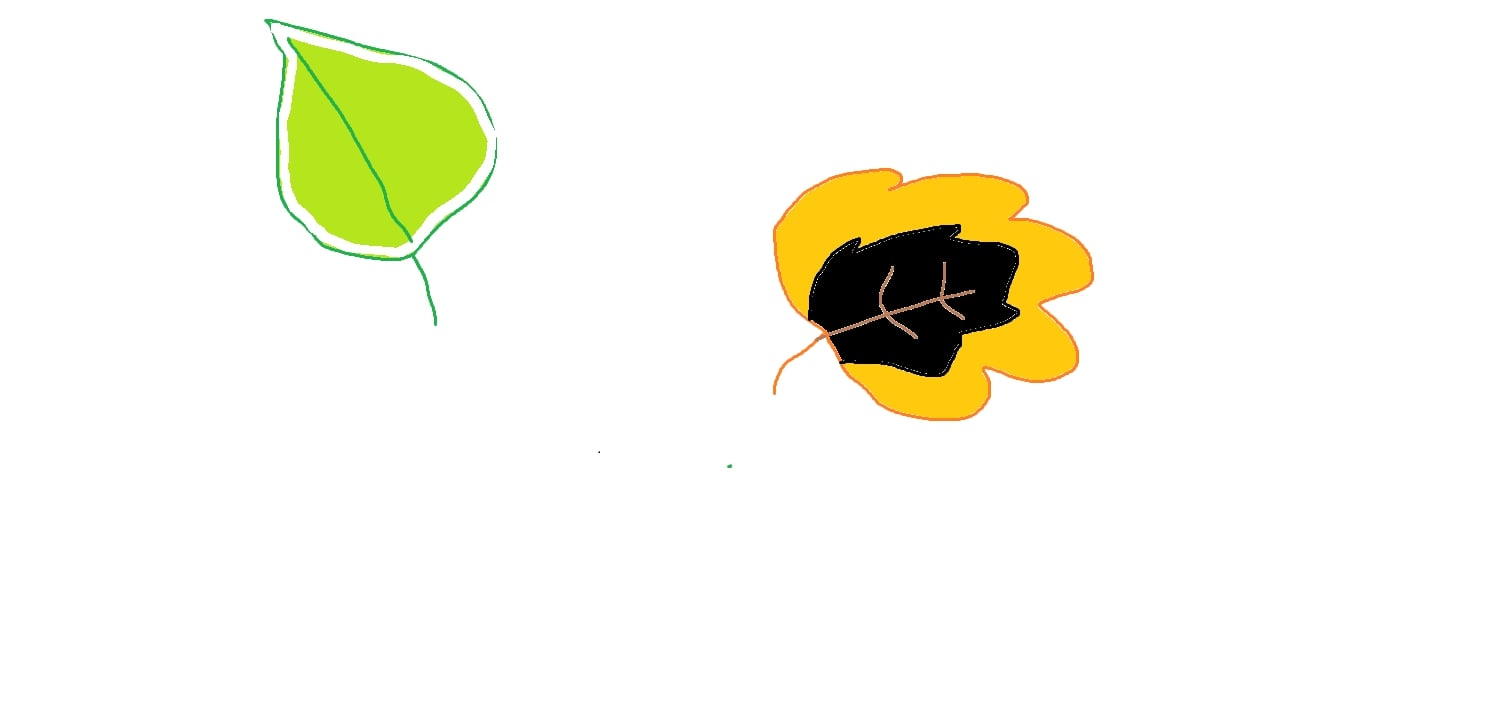
\includegraphics[width=\textwidth]{lab.jpg}
\textbf{QUESTION}
\begin{enumerate}[label=\textbf{\arabic*.}]
	\item The pattern of the black area are where the starch is. It also corresponds to where the chlorophyll was and it's evident that the chlorophyll is required to make glucose and starch.
\end{enumerate}

\subsection{Procedure 3}
\textbf{QUESTIONS}
\begin{enumerate}[label=\textbf{\arabic*.}]
	\item What is the main function of the green pigments? \\
		Chlorophyll A and Chlorophyll B compliment each other by receiving and transferring light energy which further allows plants to create oxygen.
	\item What is the main function of the pigments that aren't green? \\
		The carotenoids (Carotene \& Xanthrophyll) assist Chlorophyll by receiving wavelengths of light \textit{separate} from Chlorophyll. Also is displaying colors generally seen in the spectrum from red to yellow.
\end{enumerate}

\subsection{Procedure 4}
\textbf{Table 5.1} \\
\begin{tabular} { | c | c | c | }
	& \makecell{Number of Discs \\ Floating in Bicarbonate} & \makecell{Number of Discs  \\ Floating in Tap Water} \\
	\hline
	0 & 0 & 0 \\
	\hline
	1 & 0 & 0 \\
	\hline
	2 & 1 & 0 \\
	\hline
	3 & 1 & 0 \\
	\hline
	4 & 2 & 1 \\
	\hline
	5 & 3 & 1 \\
	\hline
	6 & 5 & 1 \\
	\hline
	7 & 7 & 2 \\
	\hline
	8 & 9 & 3 \\
	\hline
	9 & 10 & 3 \\
	\hline
	10 & 10 & 3 \\
	\hline
	11 & 10 & 3 \\
	\hline
	12 & 10 & 4 \\
	\hline
	13 & 10 & 4 \\
	\hline
	14 & 10 & 4
\end{tabular} \\
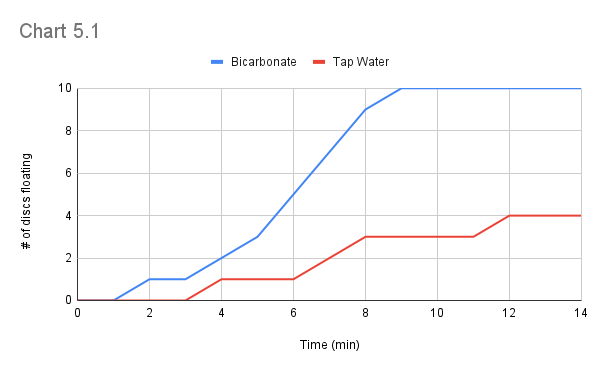
\includegraphics[width=\textwidth]{chart_5_1.png}
\textbf{QUESTIONS}
\begin{enumerate}[label=\textbf{\arabic*.}]
	\item Which syringe had the most floating disks? Why? \\
		The Sodium Bicarbonate. In order for plants to exercise photosynthesis, the plant must have a carbon source. Upon deoxygenating the spinach disks, the sample inside the water cup were unable to receive any carbon resulting in a majority to sink. Contrasted with the Sodium Bicarbonate, the spinach disks had a source of carbon which could be utilized by the spinach, and rise.
	\item What is the gas being released by the leaf disks? \\
		Per photosynthesis, the leaf disks release oxygen.
	\item Which syringe is the control? \\
		The syringe containing tap water is the control.
	\item Which syringe is the experimental? \\
		The syringe containing Sodium Bicarbonate is the experimental.
	\item What is the experimental variable in this experimental design? \\
		The solution inside the syringe would be the experimental variable.
	\item List at least two controls in this experimental design.
		\begin{enumerate}[label=\textbf{\arabic*.}]
			\item The amount of disks
			\item Lamp
		\end{enumerate}
\end{enumerate}

\end{document}
